% Chapter Template

\chapter{Desarrollo} % Main chapter title

\label{Chapter3} % Change X to a consecutive number; for referencing this chapter elsewhere, use \ref{ChapterX}

%----------------------------------------------------------------------------------------
%	SECTION 1
%----------------------------------------------------------------------------------------

\section{Introducción}

En el presente capítulo se exponen las distintas vías propuestas para abordar la resolución del problema, con el desarrollo de unos prototipos para validación de concepto. Se trata muestra, también, la evolución del prototipo hasta la versión funcional de laboratorio, así como los detalles de la versión final desarrollada y empleada en la línea de producción.

%----------------------------------------------------------------------------------------
%	SECTION 2
%----------------------------------------------------------------------------------------

\section{Prototipo de validación de concepto}

Para dar solución al problema planteado, inicialmente se realizan dos pruebas con tecnologías diferentes. Por un lado, y por petición de la empresa, se presentó una versión basada en visión por computador, tecnología utilizada por el autor del presente proyecto en proyectos anteriores. Por otra parte, se dió una solución alternativa basada en sensores giróscopo-acelerómetro.

%-----------------------------------
%	SUBSECTION 1
%-----------------------------------
\subsection{Cámara visión por computador}

Se realiza una prueba piloto aprovechando el sistema de visión instalado para otro proyecto, compuesto por la cámara fija de Fanuc, 2 paneles LED de luz difusa (60W) y el software de visión Fanuc: iRvision. Se elige realizar las pruebas en ésta plataforma, y no en un ordenador convencional con matlab u opencv, por inmediatez, el sistema está ya calibrado y en funcionamiento, además de que cuenta con un rack de salidas y entradas digitales; como se ha dicho, el objetivo era comprobar la viabilidad.

El sistema de visión está conectado al controlador de un brazo robótico LRMate 200iD, con un módulo I/O digitales a 24 voltios. Por lo que se realiza una interfaz con 2 relés para comunicar con la placa Arduino (5V), empleada para mover y calibrar los servos del juguete. En la figura \ref{fig:CeldaFanuc}

\begin{figure}[th]
\centering
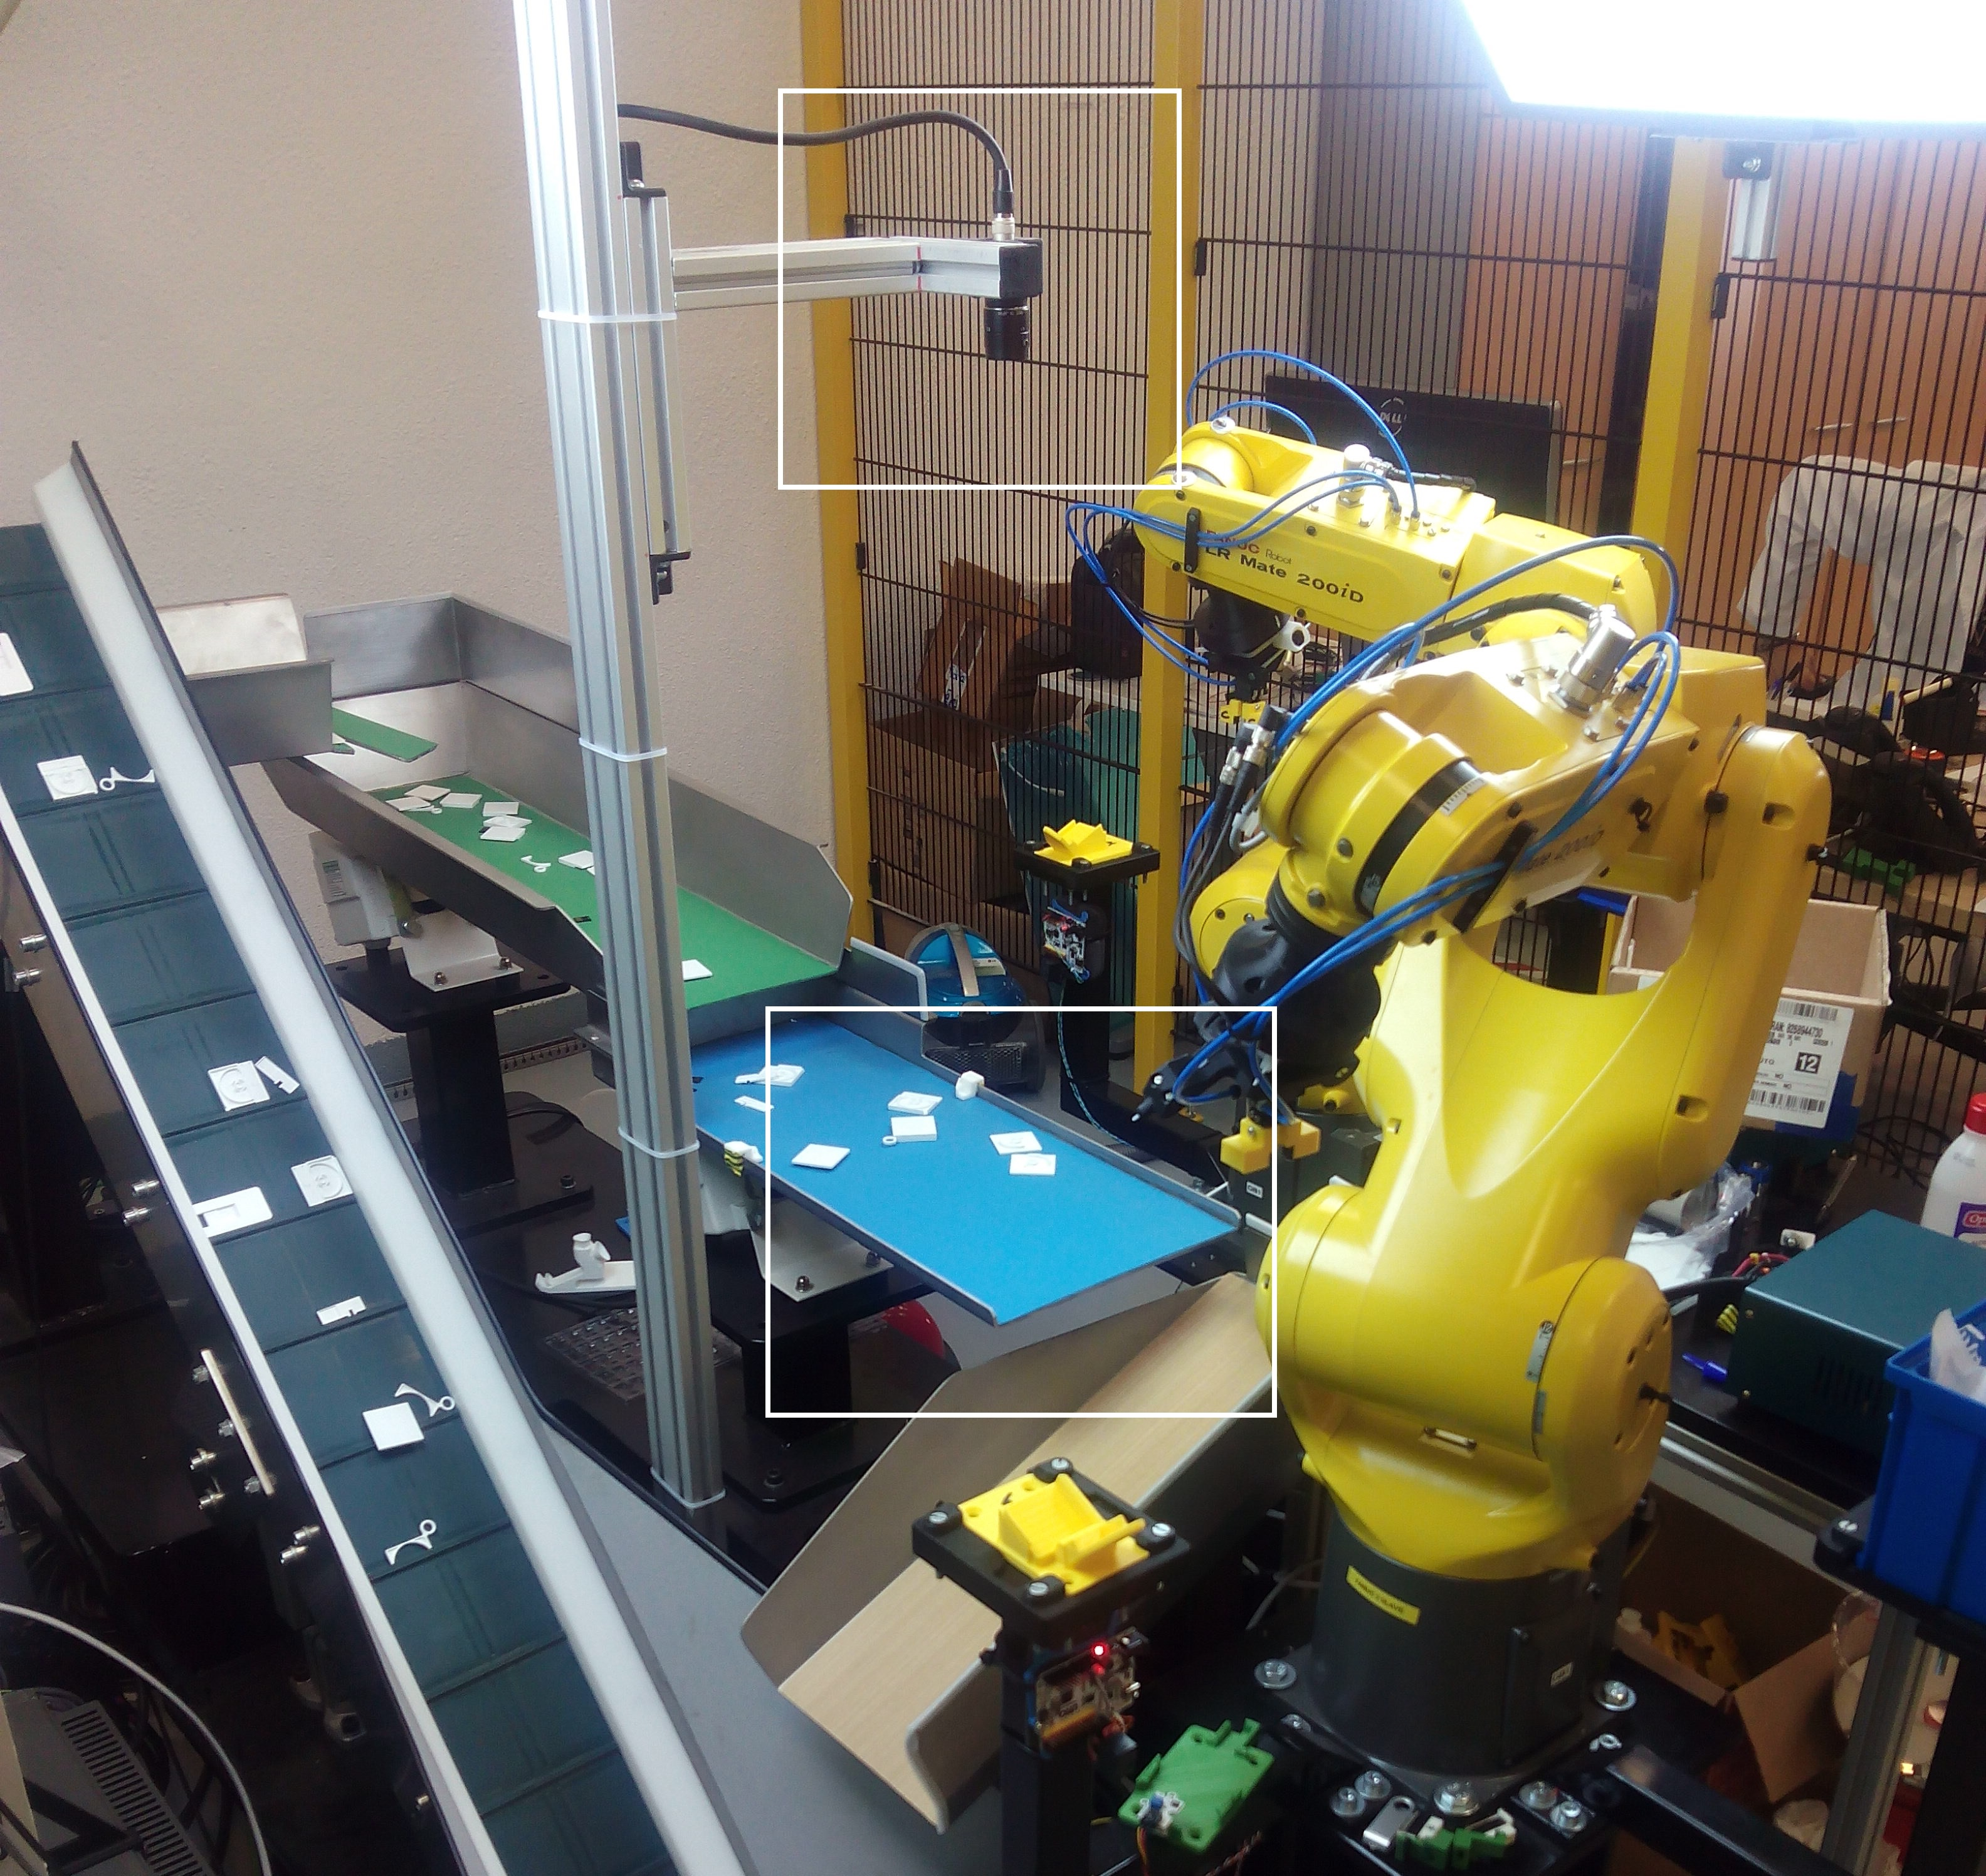
\includegraphics[width=100mm]{Figures/CeldaFanuc}
\decoRule
\caption[Celda cámara visión]{Celda con cámara de Fanuc}
\label{fig:CeldaFanuc}
\end{figure}
%-----------------------------------
%	SUBSECTION 2
%-----------------------------------

\subsection{Sensores IMUs}
Morbi rutrum odio eget arcu adipiscing sodales. Aenean et purus a est pulvinar pellentesque. Cras in elit neque, quis varius elit. Phasellus fringilla, nibh eu tempus venenatis, dolor elit posuere quam, quis adipiscing urna leo nec orci. Sed nec nulla auctor odio aliquet consequat. Ut nec nulla in ante ullamcorper aliquam at sed dolor. Phasellus fermentum magna in augue gravida cursus. Cras sed pretium lorem. Pellentesque eget ornare odio. Proin accumsan, massa viverra cursus pharetra, ipsum nisi lobortis velit, a malesuada dolor lorem eu neque.


%-----------------------------------
%	Conclusiones
%-----------------------------------

\subsection{Conclusiones}
Morbi rutrum odio eget arcu adipiscing sodales. Aenean et purus a est pulvinar pellentesque. Cras in elit neque, quis varius elit. Phasellus fringilla, nibh eu tempus venenatis, dolor elit posuere quam, quis adipiscing urna leo nec orci. Sed nec nulla auctor odio aliquet consequat. Ut nec nulla in ante ullamcorper aliquam at sed dolor. Phasellus fermentum magna in augue gravida cursus. Cras sed pretium lorem. Pellentesque eget ornare odio. Proin accumsan, massa viverra cursus pharetra, ipsum nisi lobortis velit, a malesuada dolor lorem eu neque.

%----------------------------------------------------------------------------------------
%	SECTION 3: Laboratorio
%----------------------------------------------------------------------------------------

\section{Prototipo de laboratorio}

Sed ullamcorper quam eu nisl interdum at interdum enim egestas. Aliquam placerat justo sed lectus lobortis ut porta nisl porttitor. Vestibulum mi dolor, lacinia molestie gravida at, tempus vitae ligula. Donec eget quam sapien, in viverra eros. Donec pellentesque justo a massa fringilla non vestibulum metus vestibulum. Vestibulum in orci quis felis tempor lacinia. Vivamus ornare ultrices facilisis. Ut hendrerit volutpat vulputate. Morbi condimentum venenatis augue, id porta ipsum vulputate in. Curabitur luctus tempus justo. Vestibulum risus lectus, adipiscing nec condimentum quis, condimentum nec nisl. Aliquam dictum sagittis velit sed iaculis. Morbi tristique augue sit amet nulla pulvinar id facilisis ligula mollis. Nam elit libero, tincidunt ut aliquam at, molestie in quam. Aenean rhoncus vehicula hendrerit.

%-----------------------------------
%	SUBSECTION 1
%-----------------------------------
\subsection{Subsection 1}

Nunc posuere quam at lectus tristique eu ultrices augue venenatis. Vestibulum ante ipsum primis in faucibus orci luctus et ultrices posuere cubilia Curae; Aliquam erat volutpat. Vivamus sodales tortor eget quam adipiscing in vulputate ante ullamcorper. Sed eros ante, lacinia et sollicitudin et, aliquam sit amet augue. In hac habitasse platea dictumst.

%-----------------------------------
%	SUBSECTION 2
%-----------------------------------

\subsection{Subsection 2}
Morbi rutrum odio eget arcu adipiscing sodales. Aenean et purus a est pulvinar pellentesque. Cras in elit neque, quis varius elit. Phasellus fringilla, nibh eu tempus venenatis, dolor elit posuere quam, quis adipiscing urna leo nec orci. Sed nec nulla auctor odio aliquet consequat. Ut nec nulla in ante ullamcorper aliquam at sed dolor. Phasellus fermentum magna in augue gravida cursus. Cras sed pretium lorem. Pellentesque eget ornare odio. Proin accumsan, massa viverra cursus pharetra, ipsum nisi lobortis velit, a malesuada dolor lorem eu neque.



%----------------------------------------------------------------------------------------
%	SECTION 4: Finales
%----------------------------------------------------------------------------------------

\section{Armarios finales}

Sed ullamcorper quam eu nisl interdum at interdum enim egestas. Aliquam placerat justo sed lectus lobortis ut porta nisl porttitor. Vestibulum mi dolor, lacinia molestie gravida at, tempus vitae ligula. Donec eget quam sapien, in viverra eros. Donec pellentesque justo a massa fringilla non vestibulum metus vestibulum. Vestibulum in orci quis felis tempor lacinia. Vivamus ornare ultrices facilisis. Ut hendrerit volutpat vulputate. Morbi condimentum venenatis augue, id porta ipsum vulputate in. Curabitur luctus tempus justo. Vestibulum risus lectus, adipiscing nec condimentum quis, condimentum nec nisl. Aliquam dictum sagittis velit sed iaculis. Morbi tristique augue sit amet nulla pulvinar id facilisis ligula mollis. Nam elit libero, tincidunt ut aliquam at, molestie in quam. Aenean rhoncus vehicula hendrerit.

%-----------------------------------
%	SUBSECTION 1
%-----------------------------------
\subsection{Subsection 1}

Nunc posuere quam at lectus tristique eu ultrices augue venenatis. Vestibulum ante ipsum primis in faucibus orci luctus et ultrices posuere cubilia Curae; Aliquam erat volutpat. Vivamus sodales tortor eget quam adipiscing in vulputate ante ullamcorper. Sed eros ante, lacinia et sollicitudin et, aliquam sit amet augue. In hac habitasse platea dictumst.

%-----------------------------------
%	SUBSECTION 2
%-----------------------------------

\subsection{Subsection 2}
Morbi rutrum odio eget arcu adipiscing sodales. Aenean et purus a est pulvinar pellentesque. Cras in elit neque, quis varius elit. Phasellus fringilla, nibh eu tempus venenatis, dolor elit posuere quam, quis adipiscing urna leo nec orci. Sed nec nulla auctor odio aliquet consequat. Ut nec nulla in ante ullamcorper aliquam at sed dolor. Phasellus fermentum magna in augue gravida cursus. Cras sed pretium lorem. Pellentesque eget ornare odio. Proin accumsan, massa viverra cursus pharetra, ipsum nisi lobortis velit, a malesuada dolor lorem eu neque.
